\documentclass{beamer}
\usepackage{tikz,amsmath,hyperref,graphicx,stackrel,animate,tipa,listings}
\usetikzlibrary{positioning,shadows,arrows,shapes,calc}
\newcommand{\ipa}[1]{\fontfamily{cmr}\selectfont\textipa{#1}}
\newcommand{\best}{\operatornamewithlimits{best}}
\newcommand{\argbest}{\operatornamewithlimits{argbest}}
\newcommand{\argmax}{\operatornamewithlimits{argmax}}
\newcommand{\argmin}{\operatornamewithlimits{argmin}}
\newcommand{\logsumexp}{\operatornamewithlimits{logsumexp}}
\mode<presentation>{\usetheme{Frankfurt}}
\DeclareMathOperator*{\softmax}{softmax}
\AtBeginSection[]
{
  \begin{frame}<beamer>
    \frametitle{Outline}
    \tableofcontents[currentsection,currentsubsection]
  \end{frame}
}
\title{Lecture 15: Weighted Finite State Acceptors (WFSA)}
\author{Mark Hasegawa-Johnson\\All content~\href{https://creativecommons.org/licenses/by-sa/4.0/}{CC-SA 4.0} unless otherwise specified.}
\date{ECE 417: Multimedia Signal Processing, Fall 2020}  
\begin{document}

% Title
\begin{frame}
  \maketitle
\end{frame}

% Title
\begin{frame}
  \tableofcontents
\end{frame}

%%%%%%%%%%%%%%%%%%%%%%%%%%%%%%%%%%%%%%%%%%%%
\section[Review]{Review: Hidden Markov Models}
\setcounter{subsection}{1}

\begin{frame}
  \frametitle{The Three Problems for an HMM}
   \begin{center}
    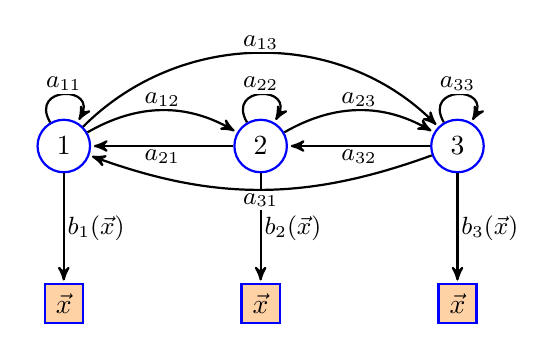
\begin{tikzpicture}[->,>=stealth',shorten >=1pt,auto,node distance=3cm,thick,
        state/.style={circle,thick,draw=blue,text=black,text centered,text width=0.25cm},
        obs/.style={rectangle,thick,draw=blue,text=black,fill=orange!35!white,text centered,text width=0.25cm}
      ]
      \node[state] (q1) at (0,0) {1};
      \node[state] (q2) at (2.5,0) {2};
      \node[state] (q3) at (5,0) {3};
      \node[obs] (x1) at (0,-2) {$\vec{x}$};
      \node[obs] (x2) at (2.5,-2) {$\vec{x}$};
      \node[obs] (x3) at (5,-2) {$\vec{x}$};
      \path[every node/.style={font=\sffamily\small,
  	  fill=white,inner sep=1pt}]
      (q1) edge [out=120,in=60,looseness=4] node {$a_{11}$} (q1)
      edge [out=30,in=150] node {$a_{12}$} (q2)
      edge [out=45,in=135] node {$a_{13}$} (q3)
      edge [out=-90,in=90] node {$b_1(\vec{x})$} (x1)
      (q2) edge [out=120,in=60,looseness=4] node {$a_{22}$} (q2)
      edge [out=180,in=0] node {$a_{21}$} (q1)
      edge [out=30,in=150] node {$a_{23}$} (q3)
      edge [out=-90,in=90] node {$b_2(\vec{x})$} (x2)
      (q3) edge [out=120,in=60,looseness=4] node {$a_{33}$} (q3)
      edge [out=180,in=0] node {$a_{32}$} (q2)
      edge [out=-160,in=-20] node {$a_{31}$} (q1)
      edge [out=-90,in=90] node {$b_3(\vec{x})$} (x3);
    \end{tikzpicture}
  \end{center}
  \begin{itemize}
  \item $\pi_i = p(q_1=i)$ is called the {\bf initial state probability}.
  \item $a_{ij} = p(q_t=j|q_{t-1}=i)$ is called the {\bf transition
    probability}.
  \item $b_j(\vec{x}) = p(\vec{x}_t=\vec{x}|q_t=j)$ is called the
    {\bf observation probability}.
  \end{itemize}
\end{frame}

\begin{frame}
  \frametitle{Recognition: The Forward Algorithm}

  \begin{enumerate}
  \item {\bf Initialize:}
    \[
    \alpha_1(i) = \pi_i b_i(\vec{x}_1)
    \]
  \item {\bf Iterate:}
    \begin{align*}
      \alpha_{t}(j) &=
      \sum_{i=1}^N p(q_{t-1}=i|\vec{x}_1,\ldots,\vec{x}_{t-1})a_{ij}b_j(\vec{x}_t)\\
      &=\sum_{i=1}^N \hat\alpha_{t-1}(i) a_{ij}b_j(\vec{x}_t)
    \end{align*}
  \item {\bf Terminate:}
    \[
    \ln p(X|\Lambda) = \sum_{j=1}^N \alpha_T(j)
    \]
  \end{enumerate}
\end{frame}

\begin{frame}
  \frametitle{Segmentation: The Log-Viterbi Algorithm}

  \begin{enumerate}
  \item {\bf Initialize:}
    \[
    \ln\delta_1(i) = \ln\pi_i +\ln b_i(\vec{x}_1)
    \]
  \item {\bf Iterate:}
    \begin{align*}
      \ln\delta_{t}(j) &= \max_{i=1}^N\left(\ln\delta_{t-1}(i) +\ln a_{ij}+ \ln b_j(\vec{x}_t)\right)\\
      \psi_{t}(j) &= \argmax_{i=1}^N\left(\ln\delta_{t-1}(i) +\ln a_{ij}+ \ln b_j(\vec{x}_t)\right)
    \end{align*}
  \item {\bf Terminate:}
    Choose the known final state $q_T^*$.
  \item {\bf Backtrace:}
    \begin{align*}
      q_t^* &= \psi_{t+1}\left(q_{t+1}^*\right)
    \end{align*}
  \end{enumerate}
\end{frame}


%%%%%%%%%%%%%%%%%%%%%%%%%%%%%%%%%%%%%%%%%%%%
\section[WFSA]{Weighted Finite State Acceptors}
\setcounter{subsection}{1}

\begin{frame}
  \frametitle{Finite State Acceptors}

  All of the material in today's lecture comes from this article:
  \centerline{\includegraphics[height=2.5in]{mohri_title.png}}
\end{frame}

\begin{frame}
  \frametitle{Finite State Acceptors}
  \begin{center}
    \tikzstyle{state}=[circle,thin,draw=blue,text width=0.25cm,fill=white]
    \tikzstyle{initial}=[circle,thick,draw=blue,text width=0.25cm,fill=white]
    \tikzstyle{final}=[circle,double,draw=blue,text width=0.25cm,fill=white]    
    \begin{tikzpicture}[->,>=stealth',shorten >=1pt,auto,node distance=3cm,thick]
      \node[initial] (q0) at (0,0) {0};
      \node[state] (q1) at (2,1) {1};
      \node[state] (q2) at (2,-1) {2};
      \node[state] (q3) at (4,0) {3};
      \node[state] (q4) at (6,0) {4};
      \node[final] (q5) at (8,0) {5};
      \node[final] (q6) at (8,-1) {6};
      \path[every node/.style={font=\sffamily\small,
  	  fill=white,inner sep=1pt}]
      (q0) edge [out=60,in=135] node {The} (q1)
      edge [out=30,in=-135] node {A} (q1)
      edge [out=-30,in=135] node {A} (q2)
      edge [out=-135,in=-135] node {This} (q2)
      (q1) edge [out=0,in=135] node {dog} (q3)
      (q2) edge [out=45,in=180] node {dog} (q3)
      edge [out=-45,in=-135] node {cat} (q3)
      (q3) edge node {is} (q4)
      (q4) edge [out=120,in=60,looseness=4] node {very} (q4)
      edge [out=0,in=180] node {cute} (q5)
      edge [out=-45,in=180] node {hungry} (q6);
    \end{tikzpicture}
  \end{center}
  
  A {\bf Finite State Acceptor (FSA)},
  $A=\left\{\Sigma,Q,E,i,F\right\}$, is a finite state machine capable
  of accepting any string in a (possibly infinite) set.
  \begin{itemize}
  \item $Q$ is a set of states, and $E$ a set of edges.
  \item $\Sigma$ is an alphabet of labels that
    may appear on edges.
  \item $i$ is the initial state, shown with a thick border.  $F$ is
    the set of final states, shown with doubled borders.
  \end{itemize}
\end{frame}

\begin{frame}
  \frametitle{Weighted Finite State Acceptors}
  \begin{center}
    \tikzstyle{state}=[circle,thin,draw=blue,text width=0.25cm,fill=white]
    \tikzstyle{initial}=[circle,thick,draw=blue,text width=0.25cm,fill=white]
    \tikzstyle{final}=[circle,double,draw=blue,text width=0.25cm,fill=white]    
    \begin{tikzpicture}[->,>=stealth',shorten >=1pt,auto,node distance=3cm,thick]
      \node[initial] (q0) at (0,0) {0};
      \node[state] (q1) at (2,1) {1};
      \node[state] (q2) at (2,-1) {2};
      \node[state] (q3) at (4,0) {3};
      \node[state] (q4) at (6,0) {4};
      \node[final,label=right:$0.3$] (q5) at (8,0) {5};
      \node[final,label=right:$0.7$] (q6) at (8,-1) {6};
      \path[every node/.style={font=\sffamily\small,
  	  fill=white,inner sep=1pt}]
      (q0) edge [out=60,in=135] node {The/$0.3$} (q1)
      edge [out=30,in=-135] node {A/$0.2$} (q1)
      edge [out=-45,in=180] node {A/$0.3$} (q2)
      edge [out=-135,in=-135] node {This/$0.2$} (q2)
      (q1) edge [out=0,in=135] node {dog/$1$} (q3)
      (q2) edge [out=45,in=180] node {dog/$0.3$} (q3)
      edge [out=-45,in=-90] node {cat/$0.7$} (q3)
      (q3) edge node {is/$1$} (q4)
      (q4) edge [out=120,in=60,looseness=4] node {very/$0.2$} (q4)
      edge [out=0,in=180] node {cute/$0.4$} (q5)
      edge [out=-45,in=180] node {hungry/$0.4$} (q6);
    \end{tikzpicture}
  \end{center}
  
  A {\bf Weighted Finite State Acceptor (WFSA)} is an FSA with weights
  on the edges.
  \begin{itemize}
  \item The edge weights are usually interpreted as conditional probabilities (of the
    edge given the state), but other interpretations are possible.
  \item It's also possible to put probabilities on the final states,
    as shown in this figure (but we don't do this very often).
  \end{itemize}
\end{frame}

\begin{frame}
  \frametitle{What it's for}
  \begin{itemize}
  \item An {\bf FSA} specifies a set of strings.  A string is in the set if
    it corresponds to a valid path from start to end, and not otherwise.
  \item A {\bf WFSA} also specifies a probability mass function over the set.
  \end{itemize}
\end{frame}

\begin{frame}
  \frametitle{Every Markov Model is a WFSA}
  \begin{center}
    \tikzstyle{state}=[circle,thin,draw=blue,text width=0.25cm,fill=white]
    \tikzstyle{initial}=[circle,thick,draw=blue,text width=0.25cm,fill=white]
    \tikzstyle{final}=[circle,double,draw=blue,text width=0.25cm,fill=white]    
    \begin{tikzpicture}[->,>=stealth',shorten >=1pt,auto,node distance=3cm,thick]
      \node[initial] (q1) at (0,0) {1};
      \node[state] (q2) at (3,0) {2};
      \node[final] (q3) at (6,0) {3};
      \path[every node/.style={font=\sffamily\small,
  	  fill=white,inner sep=1pt}]
      (q1) edge [out=-120,in=120,looseness=4] node {1/$a_{11}$} (q1)
      edge [out=15,in=165] node {1/$a_{12}$} (q2)
      edge [out=45,in=135] node {1/$a_{13}$} (q3)
      (q2) edge [out=120,in=60,looseness=4] node {2/$a_{22}$} (q2)
      edge [out=-165,in=-15] node {2/$a_{21}$} (q1)
      edge [out=15,in=165] node {2/$a_{23}$} (q3)
      (q3) edge [out=60,in=-60,looseness=4] node {3/$a_{33}$} (q3)
      edge [out=-165,in=-15] node {3/$a_{32}$} (q2)
      edge [out=-135,in=-45] node {3/$a_{31}$} (q1);
    \end{tikzpicture}
  \end{center}
  A Markov Model (but not an HMM!) may be interpreted as a WFSA: just
  assign a label to each edge.  The label might just be the state
  number, or it might be something more useful.
\end{frame}
  
%%%%%%%%%%%%%%%%%%%%%%%%%%%%%%%%%%%%%%%%%%%%
\section[Multiplication]{Multiplication}
\setcounter{subsection}{1}

\begin{frame}
  \frametitle{Multiplication: Accumulate on a Path}
  \begin{center}
    \tikzstyle{state}=[circle,thin,draw=blue,text width=0.25cm,fill=white]
    \tikzstyle{initial}=[circle,thick,draw=blue,text width=0.25cm,fill=white]
    \tikzstyle{final}=[circle,double,draw=blue,text width=0.25cm,fill=white]    
    \begin{tikzpicture}[->,>=stealth',shorten >=1pt,auto,node distance=3cm,thick]
      \node[initial] (q0) at (0,0) {0};
      \node[state] (q1) at (2,1) {1};
      \node[state] (q2) at (2,-1) {2};
      \node[state] (q3) at (4,0) {3};
      \node[state] (q4) at (6,0) {4};
      \node[final] (q5) at (8,0) {5};
      \node[final] (q6) at (8,-1) {6};
      \path[every node/.style={font=\sffamily\small,
  	  fill=white,inner sep=1pt}]
      (q0) edge [out=60,in=135] node {The/$0.3$} (q1)
      edge [out=30,in=-135] node {A/$0.2$} (q1)
      edge [out=-45,in=180] node {A/$0.3$} (q2)
      edge [out=-135,in=-135] node {This/$0.2$} (q2)
      (q1) edge [out=0,in=135] node {dog/$1$} (q3)
      (q2) edge [out=45,in=180] node {dog/$0.3$} (q3)
      edge [out=-45,in=-90] node {cat/$0.7$} (q3)
      (q3) edge node {is/$1$} (q4)
      (q4) edge [out=120,in=60,looseness=4] node {very/$0.2$} (q4)
      edge [out=0,in=180] node {cute/$0.4$} (q5)
      edge [out=-45,in=180] node {hungry/$0.4$} (q6);
    \end{tikzpicture}
  \end{center}
  
  {\bf Multiplication} is used to accumulate the weights on a single
  path through the WFSA.  For example, there are two paths matching
  the sentence ``A dog is hungry''  Their path weights are
  \begin{align*}
    p(\mbox{Path through state 1}) &= (0.2)(1)(1)(0.4) = 0.08\\
    p(\mbox{Path through state 2}) &= (0.3)(0.3)(1)(0.4) = 0.036
  \end{align*}
\end{frame}

\begin{frame}
  \frametitle{Negative Log Probabilities}

  WFSAs have floating point underflow problems.  The standard solution
  is to perform all computations using negative log probabilities.
  Negative log probability ($-\log p(A)$) goes by many names:
  \begin{itemize}
  \item ``Surprisal,'' because you are more surprised if something
    unlikely happens.
  \item ``Information,'' because low-probability events are more informative.
  \item ``Cost,'' because it costs more to take a low-probability path.
  \end{itemize}
\end{frame}

\begin{frame}
  \frametitle{WFSA with Negative Log Probabilities}
  \begin{center}
    \tikzstyle{state}=[circle,thin,draw=blue,text width=0.25cm,fill=white]
    \tikzstyle{initial}=[circle,thick,draw=blue,text width=0.25cm,fill=white]
    \tikzstyle{final}=[circle,double,draw=blue,text width=0.25cm,fill=white]    
    \begin{tikzpicture}[->,>=stealth',shorten >=1pt,auto,node distance=3cm,thick]
      \node[initial] (q0) at (0,0) {0};
      \node[state] (q1) at (2,1) {1};
      \node[state] (q2) at (2,-1) {2};
      \node[state] (q3) at (4,0) {3};
      \node[state] (q4) at (6,0) {4};
      \node[final] (q5) at (8,0) {5};
      \node[final] (q6) at (8,-1) {6};
      \path[every node/.style={font=\sffamily\small,
  	  fill=white,inner sep=1pt}]
      (q0) edge [out=60,in=135] node {The/$1.2$} (q1)
      edge [out=30,in=-135] node {A/$1.6$} (q1)
      edge [out=-45,in=180] node {A/$1.2$} (q2)
      edge [out=-135,in=-135] node {This/$1.6$} (q2)
      (q1) edge [out=0,in=135] node {dog/$0$} (q3)
      (q2) edge [out=45,in=180] node {dog/$1.2$} (q3)
      edge [out=-45,in=-90] node {cat/$0.4$} (q3)
      (q3) edge node {is/$0$} (q4)
      (q4) edge [out=120,in=60,looseness=4] node {very/$1.6$} (q4)
      edge [out=0,in=180] node {cute/$0.9$} (q5)
      edge [out=-45,in=180] node {hungry/$0.9$} (q6);
    \end{tikzpicture}
  \end{center}
  
  {\bf Adding Negative Log Probabilities} accumulates the costs on a single
  path.  For example, there are two paths matching
  the sentence ``A dog is hungry''  Their path weights are
  \begin{align*}
    -\ln p(\mbox{Path through state 1}) &= 1.6+0+0+0.9 = 2.5\\
    -\ln p(\mbox{Path through state 2}) &= 1.2+1.2+0+0.9 = 3.3
  \end{align*}
\end{frame}

\begin{frame}
  \frametitle{Otimes Notation}

  In designing a WFSA, we want our design to be robust, even if we
  suddenly change between probabilities$\leftrightarrow$negative log
  probabilities.  Instead of using the standard
  real-valued ``times'' operator, and the constants ``1'' and ``0,''
  we use overloaded operators $\otimes$,
  $\bar{1}$, and $\bar{0}$ whose behavior is determined by the type  of their inputs:
  \begin{itemize}
  \item If the inputs are probabilities, then $\otimes$ means
    ``multiply,'' $\bar{1}$ means ``one,'' and $\bar{0}$
    means''zero.''  Thus, for example
    \begin{align*}
      (0.2)\otimes(0.7)\otimes\bar{1} &= 0.2\cdot 0.7\cdot 1 = 0.14\\
      (0.2)\otimes\bar{0} &= 0.2\cdot 0 = 0
    \end{align*}
  \item If the inputs are negative log probabilities, then $\otimes$
    means ``add,'' $\bar{1}$ means $-\ln(1)=0$, and $\bar{0}$ means $-\ln(0)=\infty$.  Thus
    \begin{align*}
      (1.6)\otimes(0.4)\otimes\bar{1} &= 1.6+0.4+0 = 2.0\\
      (1.6)\otimes\bar{0} &= 1.6+\infty = \infty
    \end{align*}
  \end{itemize}
\end{frame}

%%%%%%%%%%%%%%%%%%%%%%%%%%%%%%%%%%%%%%%%%%%%
\section[Best Path]{Best Path}
\setcounter{subsection}{1}

\begin{frame}
  \frametitle{Finding the Best Path}
  \begin{center}
    \tikzstyle{state}=[circle,thin,draw=blue,text width=0.25cm,fill=white]
    \tikzstyle{initial}=[circle,thick,draw=blue,text width=0.25cm,fill=white]
    \tikzstyle{final}=[circle,double,draw=blue,text width=0.25cm,fill=white]    
    \begin{tikzpicture}[->,>=stealth',shorten >=1pt,auto,node distance=3cm,thick]
      \node[initial] (q0) at (0,0) {0};
      \node[state] (q1) at (2,1) {1};
      \node[state] (q2) at (2,-1) {2};
      \node[state] (q3) at (4,0) {3};
      \node[state] (q4) at (6,0) {4};
      \node[final] (q5) at (8,0) {5};
      \node[final] (q6) at (8,-1) {6};
      \path[every node/.style={font=\sffamily\small,
  	  fill=white,inner sep=1pt}]
      (q0) edge [out=60,in=135] node {The/$0.3$} (q1)
      edge [out=30,in=-135] node {A/$0.2$} (q1)
      edge [out=-45,in=180] node {A/$0.3$} (q2)
      edge [out=-135,in=-135] node {This/$0.2$} (q2)
      (q1) edge [out=0,in=135] node {dog/$1$} (q3)
      (q2) edge [out=45,in=180] node {dog/$0.3$} (q3)
      edge [out=-45,in=-90] node {cat/$0.7$} (q3)
      (q3) edge node {is/$1$} (q4)
      (q4) edge [out=120,in=60,looseness=4] node {very/$0.2$} (q4)
      edge [out=0,in=180] node {cute/$0.4$} (q5)
      edge [out=-45,in=180] node {hungry/$0.4$} (q6);
    \end{tikzpicture}
  \end{center}

  Often, given an input string, we want to find the {\bf best path}
  matching that string.  This is done using a version of the Viterbi
  algorithm.
\end{frame}

\begin{frame}
  \frametitle{Best-Path Algorithm for a WFSA}

  Given:
  \begin{itemize}
  \item Input string, $S=[s_1,\ldots,s_T]$.  For example, the
    string ``A dog is very very hungry'' has $T=5$ words.
  \item Edges, $e$, each have predecessor state $p[e]\in Q$, next state
    $n[e]\in Q$, weight $w[e]\in\overline{\mathbb{R}}$ and label $\ell[e]\in\Sigma$.
  \end{itemize}
  \begin{itemize}
  \item {\bf Initialize:}
    \begin{displaymath}
      \delta_0(i) = \begin{cases}
        \bar{1} & i=\mbox{initial state}\\
        \bar{0} & \mbox{otherwise}
      \end{cases}
    \end{displaymath}
  \item {\bf Iterate:}
    \begin{align*}
      \delta_t(j) &= \best_{e:n[e]=j,\ell[e]=s_t} \delta_{t-1}(p[e]) \otimes w[e]\\
      \psi_t(j) &= \argbest_{e:n[e]=j,\ell[e]=s_t} \delta_{t-1}(p[e]) \otimes w[e]
    \end{align*}
  \item {\bf Backtrace:}
    \begin{displaymath}
      e^*_t = \psi(q^*_{t+1}),~~~~~q^*_t=p[e^*_t]
    \end{displaymath}
  \end{itemize}
\end{frame}
    
\begin{frame}
  \frametitle{Best Path: Probabilities}
  \begin{center}
    \tikzstyle{state}=[circle,thin,draw=blue,text width=0.25cm,fill=white]
    \tikzstyle{initial}=[circle,thick,draw=blue,text width=0.25cm,fill=white]
    \tikzstyle{final}=[circle,double,draw=blue,text width=0.25cm,fill=white]    
    \begin{tikzpicture}[->,>=stealth',shorten >=1pt,auto,node distance=3cm,thick]
      \node[initial] (q0) at (0,0) {0};
      \node[state] (q1) at (2,1) {1};
      \node[state] (q2) at (2,-1) {2};
      \node[state] (q3) at (4,0) {3};
      \node[state] (q4) at (6,0) {4};
      \node[final] (q5) at (8,0) {5};
      \node[final] (q6) at (8,-1) {6};
      \path[every node/.style={font=\sffamily\small,
  	  fill=white,inner sep=1pt}]
      (q0) edge [out=60,in=135] node {The/$0.3$} (q1)
      edge [out=30,in=-135] node {A/$0.2$} (q1)
      edge [out=-45,in=180] node {A/$0.3$} (q2)
      edge [out=-135,in=-135] node {This/$0.2$} (q2)
      (q1) edge [out=0,in=135] node {dog/$1$} (q3)
      (q2) edge [out=45,in=180] node {dog/$0.3$} (q3)
      edge [out=-45,in=-90] node {cat/$0.7$} (q3)
      (q3) edge node {is/$1$} (q4)
      (q4) edge [out=120,in=60,looseness=4] node {very/$0.2$} (q4)
      edge [out=0,in=180] node {cute/$0.4$} (q5)
      edge [out=-45,in=180] node {hungry/$0.4$} (q6);
    \end{tikzpicture}
  \end{center}

  After the first two words, ``A dog\ldots'' we have to compare two possible paths:
  \begin{displaymath}
    \delta_2(3) = \best\left(0.2\otimes 1,0.3\otimes 0.3\right) = \best\left(0.2,0.09\right)=0.2
  \end{displaymath}
\end{frame}


\begin{frame}
  \frametitle{Best Path: Log Probabilities}
  \begin{center}
    \tikzstyle{state}=[circle,thin,draw=blue,text width=0.25cm,fill=white]
    \tikzstyle{initial}=[circle,thick,draw=blue,text width=0.25cm,fill=white]
    \tikzstyle{final}=[circle,double,draw=blue,text width=0.25cm,fill=white]    
    \begin{tikzpicture}[->,>=stealth',shorten >=1pt,auto,node distance=3cm,thick]
      \node[initial] (q0) at (0,0) {0};
      \node[state] (q1) at (2,1) {1};
      \node[state] (q2) at (2,-1) {2};
      \node[state] (q3) at (4,0) {3};
      \node[state] (q4) at (6,0) {4};
      \node[final] (q5) at (8,0) {5};
      \node[final] (q6) at (8,-1) {6};
      \path[every node/.style={font=\sffamily\small,
  	  fill=white,inner sep=1pt}]
      (q0) edge [out=60,in=135] node {The/$1.2$} (q1)
      edge [out=30,in=-135] node {A/$1.6$} (q1)
      edge [out=-45,in=180] node {A/$1.2$} (q2)
      edge [out=-135,in=-135] node {This/$1.6$} (q2)
      (q1) edge [out=0,in=135] node {dog/$0$} (q3)
      (q2) edge [out=45,in=180] node {dog/$1.2$} (q3)
      edge [out=-45,in=-90] node {cat/$0.4$} (q3)
      (q3) edge node {is/$0$} (q4)
      (q4) edge [out=120,in=60,looseness=4] node {very/$1.6$} (q4)
      edge [out=0,in=180] node {cute/$0.9$} (q5)
      edge [out=-45,in=180] node {hungry/$0.9$} (q6);
    \end{tikzpicture}
  \end{center}

  After the first two words, ``A dog\ldots'' we have to compare two possible paths:
  \begin{displaymath}
    \delta_2(3) = \best\left(1.6\otimes 0,1.2\otimes 1.2\right) = \best\left(1.6,2.4\right)=1.6
  \end{displaymath}
\end{frame}


%%%%%%%%%%%%%%%%%%%%%%%%%%%%%%%%%%%%%%%%%%%%
\section[Addition]{Addition}
\setcounter{subsection}{1}

\begin{frame}
  \frametitle{Addition: Combine Paths}
  \begin{center}
    \tikzstyle{state}=[circle,thin,draw=blue,text width=0.25cm,fill=white]
    \tikzstyle{initial}=[circle,thick,draw=blue,text width=0.25cm,fill=white]
    \tikzstyle{final}=[circle,double,draw=blue,text width=0.25cm,fill=white]    
    \begin{tikzpicture}[->,>=stealth',shorten >=1pt,auto,node distance=3cm,thick]
      \node[initial] (q0) at (0,0) {0};
      \node[state] (q1) at (2,1) {1};
      \node[state] (q2) at (2,-1) {2};
      \node[state] (q3) at (4,0) {3};
      \node[state] (q4) at (6,0) {4};
      \node[final] (q5) at (8,0) {5};
      \node[final] (q6) at (8,-1) {6};
      \path[every node/.style={font=\sffamily\small,
  	  fill=white,inner sep=1pt}]
      (q0) edge [out=60,in=135] node {The/$0.3$} (q1)
      edge [out=30,in=-135] node {A/$0.2$} (q1)
      edge [out=-45,in=180] node {A/$0.3$} (q2)
      edge [out=-135,in=-135] node {This/$0.2$} (q2)
      (q1) edge [out=0,in=135] node {dog/$1$} (q3)
      (q2) edge [out=45,in=180] node {dog/$0.3$} (q3)
      edge [out=-45,in=-90] node {cat/$0.7$} (q3)
      (q3) edge node {is/$1$} (q4)
      (q4) edge [out=120,in=60,looseness=4] node {very/$0.2$} (q4)
      edge [out=0,in=180] node {cute/$0.4$} (q5)
      edge [out=-45,in=180] node {hungry/$0.4$} (q6);
    \end{tikzpicture}
  \end{center}
  
  {\bf Addition} is used to combine the weights of two different
  paths.  For example, the total probability of the sentence ``A dog
  is hungry'' is the sum of the probabilities of its two paths:
  \begin{displaymath}
    p(\mbox{A dog is hungry}) = p(\mbox{Path 1})+p(\mbox{Path 2})=0.08+0.036=0.116
  \end{displaymath}
\end{frame}

\begin{frame}
  \frametitle{The Oplus Operator}

  When we convert from probabilities to surprisals, instead of using
  ordinary (multiplication,addition,1,0), we want to use
  overloaded operators ($\otimes$,$\oplus$,$\bar{1}$,$\bar{0}$),
  whose behavior is determined by the type of their inputs:
  \begin{itemize}
  \item If the WFSA is using probability, then $\oplus$ means
    ``addition,'' and $\bar{0}$ means ``zero.''  Thus, for example
    \begin{displaymath}
      (0.08)\oplus(0.06)\oplus\bar{0} = 0.08+0.06+0 = 0.14
    \end{displaymath}
  \item If the WFSA is using negative log probability, then $\oplus$
    and $\bar{0}$ should be redefined in some way that gives the
    desired result.  The desired  result is that:
    \begin{displaymath}
      \left(-\ln(0.08)\right)\oplus\left(-\ln(0.06)\right)\oplus\bar{0} = -\ln(0.14)
    \end{displaymath}
  \end{itemize}
\end{frame}

\begin{frame}
  \frametitle{The Negative Logsumexp Function}

  Suppose $a$ and $b$ are negative log probabilities:
  \begin{displaymath}
    a=-\ln p(A),~~~b=-\ln p(B)
  \end{displaymath}
  The most computationally efficient way to implement the $\oplus$
  operator is also the one that's easiest to understand:
  \begin{displaymath}
    a\oplus b = -\ln \left(p(A)+p(B)\right)= -\ln \left(e^{-a}+e^{-b}\right)
  \end{displaymath}
  This function is used so often, in machine learning, that it has a
  special name.  It is called the {\tt logsumexp} function:
  \begin{displaymath}
    a\oplus b = -\logsumexp(-a,-b) = -\ln \left(e^{-a}+e^{-b}\right)
  \end{displaymath}
\end{frame}

\begin{frame}
  \frametitle{Logsumexp and Floating Point Underflow}

  The most computationally efficient way to implement {\tt logsumexp}
  is also the easiest to understand.  It is just:
  \begin{displaymath}
    \logsumexp(x,y) = \ln \left(e^{x}+e^{y}\right)
  \end{displaymath}
  Unfortunately, that formula may suffer from floating point
  overflow, e.g., if $x>100$ or $y>100$.  The following
  alternative implementation is guaranteed to  avoid floating point overflow:
  \begin{align*}
    m &= \max(x,y)\\
    \logsumexp(x,y) &= m +\ln \left(e^{x-m}+e^{y-m}\right)
  \end{align*}
\end{frame}

\begin{frame}
  \frametitle{Logsumexp and Max}

  The following implementation of {\tt logsumexmp} avoids floating
  point overflow:
  \begin{align*}
    m &= \max(x,y)\\
    \logsumexp(x,y) &= m +\ln \left(e^{x-m}+e^{y-m}\right)
  \end{align*}
  For example, suppose $x>y$, then we get $\logsumexp(x,y) = x +\ln
  \left(1+e^{y-x}\right)$.  The second term inside the parentheses is
  $0\le e^{y-x}\le 1$, so
  \begin{displaymath}
    \max(x,y) \le \logsumexp(x,y) \le \max(x,y)+\ln(2)
  \end{displaymath}
  For this reason, $\logsumexp$ is a differentiable approximation of
  the $\max$ operator.
\end{frame}

\begin{frame}
  \frametitle{Addition: Combine Paths}
  \begin{center}
    \tikzstyle{state}=[circle,thin,draw=blue,text width=0.25cm,fill=white]
    \tikzstyle{initial}=[circle,thick,draw=blue,text width=0.25cm,fill=white]
    \tikzstyle{final}=[circle,double,draw=blue,text width=0.25cm,fill=white]    
    \begin{tikzpicture}[->,>=stealth',shorten >=1pt,auto,node distance=3cm,thick]
      \node[initial] (q0) at (0,0) {0};
      \node[state] (q1) at (2,1) {1};
      \node[state] (q2) at (2,-1) {2};
      \node[state] (q3) at (4,0) {3};
      \node[state] (q4) at (6,0) {4};
      \node[final] (q5) at (8,0) {5};
      \node[final] (q6) at (8,-1) {6};
      \path[every node/.style={font=\sffamily\small,
  	  fill=white,inner sep=1pt}]
      (q0) edge [out=60,in=135] node {The/$1.2$} (q1)
      edge [out=30,in=-135] node {A/$1.6$} (q1)
      edge [out=-45,in=180] node {A/$1.2$} (q2)
      edge [out=-135,in=-135] node {This/$1.6$} (q2)
      (q1) edge [out=0,in=135] node {dog/$0$} (q3)
      (q2) edge [out=45,in=180] node {dog/$1.2$} (q3)
      edge [out=-45,in=-90] node {cat/$0.4$} (q3)
      (q3) edge node {is/$0$} (q4)
      (q4) edge [out=120,in=60,looseness=4] node {very/$1.6$} (q4)
      edge [out=0,in=180] node {cute/$0.9$} (q5)
      edge [out=-45,in=180] node {hungry/$0.9$} (q6);
    \end{tikzpicture}
  \end{center}
  
  {\bf Negative Logsumexp} is used to combine the surprisals of two different
  paths.  For example, the total surprisal of the sentence ``A dog
  is hungry'' is the negative logsumexp of the surprisals of its two paths:
  \begin{align*}
    p(\mbox{A dog is hungry}) &= \left(1.6\otimes 0\otimes 0\otimes 0.9\right)\oplus\left(1.2\otimes 1.2\otimes 0\otimes 0.9\right)\\
    &=2.5\oplus 3.3 = 2.2
  \end{align*}
\end{frame}

\begin{frame}
  \frametitle{$\bar{0}$: The identity element of $\oplus$}

  The $\oplus$ operator, for surprisal weights, is a negative
  logsumexp:
  \begin{displaymath}
    a\oplus b = -\logsumexp(-a,-b) \le \min(a,b)
  \end{displaymath}
  The identity element, $\bar{0}$, is the element such that
  \begin{displaymath}
    a\oplus \bar{0} = a
  \end{displaymath}
  If you work through the definition of the $\logsumexp$ function, you
  can discover that its identity element is
  \begin{displaymath}
    \bar{0} = -\ln(0)  = +\infty
  \end{displaymath}
\end{frame}

%%%%%%%%%%%%%%%%%%%%%%%%%%%%%%%%%%%%%%%%%%%%
\section[Determinization]{Determinization}
\setcounter{subsection}{1}

\begin{frame}
  \frametitle{Determinization}

  \begin{itemize}
    \item A WFSA is said to be {\bf deterministic} if, for any given
      (predecessor state $p[e]$, label $\ell[e]$), there is at most 
      one such edge.
    \item If a WFSA is deterministic, then for any given string
      $S=[s_1,\ldots,s_T]$, there is {\bf at most one} path.
    \item Determinism makes many other computations very efficient.
      For example, the best-path algorithm is ${\mathcal
        O}\left\{T\right\}$.
  \end{itemize}
\end{frame}

\begin{frame}
  \frametitle{A Non-Deterministic WFSA: Example}

  This WFSA is not deterministic, because there are two different
  paths leaving state $p[e]=0$ that both have the label
  $\ell[e]=\mbox{``A''}$:
  \begin{center}
    \tikzstyle{state}=[circle,thin,draw=blue,text width=0.25cm,fill=white]
    \tikzstyle{initial}=[circle,thick,draw=blue,text width=0.25cm,fill=white]
    \tikzstyle{final}=[circle,double,draw=blue,text width=0.25cm,fill=white]    
    \begin{tikzpicture}[->,>=stealth',shorten >=1pt,auto,node distance=3cm,thick]
      \node[initial] (q0) at (0,0) {0};
      \node[state] (q1) at (2,1) {1};
      \node[state] (q2) at (2,-1) {2};
      \node[state] (q3) at (4,0) {3};
      \node[state] (q4) at (6,0) {4};
      \node[final] (q5) at (8,0) {5};
      \node[final] (q6) at (8,-1) {6};
      \path[every node/.style={font=\sffamily\small,
  	  fill=white,inner sep=1pt}]
      (q0) edge [out=60,in=135] node {The/$0.3$} (q1)
      edge [out=30,in=-135] node {A/$0.2$} (q1)
      edge [out=-45,in=180] node {A/$0.3$} (q2)
      edge [out=-135,in=-135] node {This/$0.2$} (q2)
      (q1) edge [out=0,in=135] node {dog/$1$} (q3)
      (q2) edge [out=45,in=180] node {dog/$0.3$} (q3)
      edge [out=-45,in=-90] node {cat/$0.7$} (q3)
      (q3) edge node {is/$1$} (q4)
      (q4) edge [out=120,in=60,looseness=4] node {very/$0.2$} (q4)
      edge [out=0,in=180] node {cute/$0.4$} (q5)
      edge [out=-45,in=180] node {hungry/$0.4$} (q6);
    \end{tikzpicture}
  \end{center}
\end{frame}

\begin{frame}
  \frametitle{Determinizing a WFSA}

  {\bf Determinizing} a WFSA is the creation of a new WFSA such that:
  \begin{itemize}
  \item If $A$ has one or more paths matching any given string,
    $S=[s_1,\ldots,s_T]$, then $A'$ must have exactly one such path.
  \item The path weight (probability, surprisal) in $A'$ must be the
    sum ($\oplus$) of the weights of all of the paths in $A$.
  \end{itemize}

\end{frame}

\begin{frame}
  \frametitle{How to Determinize a WFSA}

  The only general algorithm for {\bf determinizing} a WFSA is the
  following exponential-time algorithm:
  \begin{itemize}
  \item For every state in $A$, for every set of edges
    $e_1,\ldots,e_K$ that all have the same label:
    \begin{itemize}
    \item Create a new edge, $e$, with weight $w[e]=w[e_1]\oplus\cdots\oplus w[e_K]$.
    \item Create a brand new successor state $n[e]$.
    \item For every edge leaving any of the original successor states
      $n[e_k],~1\le k\le K$, whose label is unique:
      \begin{itemize}
      \item Copy  it to $n[e]$, $\otimes$ its weight by $w[e_k]/w[e]$
      \end{itemize}
    \item For every set of edges leaving $n[e_k]$ that all have the
      same label:
      \begin{itemize}
      \item Recurse!
      \end{itemize}
    \end{itemize}
  \end{itemize}
\end{frame}

\begin{frame}
  \frametitle{How to Determinize a WFSA: Example}
  \begin{center}
    \tikzstyle{state}=[circle,thin,draw=blue,text width=0.25cm,fill=white]
    \tikzstyle{initial}=[circle,thick,draw=blue,text width=0.25cm,fill=white]
    \tikzstyle{final}=[circle,double,draw=blue,text width=0.25cm,fill=white]    
    \begin{tikzpicture}[->,>=stealth',shorten >=1pt,auto,node distance=3cm,thick]
      \node[initial] (q0) at (0,0) {0};
      \node[state] (q1) at (2,1) {1};
      \node[state] (q2) at (2,-1) {2};
      \node[state] (q3) at (4,0) {3};
      \node[state] (q4) at (6,0) {4};
      \node[final] (q5) at (8,0) {5};
      \node[final] (q6) at (8,-1) {6};
      \path[every node/.style={font=\sffamily\small,
  	  fill=white,inner sep=1pt}]
      (q0) edge [out=60,in=135] node {The/$0.3$} (q1)
      edge [out=30,in=-135] node {A/$0.2$} (q1)
      edge [out=-45,in=180] node {A/$0.3$} (q2)
      edge [out=-135,in=-135] node {This/$0.2$} (q2)
      (q1) edge [out=0,in=135] node {dog/$1$} (q3)
      (q2) edge [out=45,in=180] node {dog/$0.3$} (q3)
      edge [out=-45,in=-90] node {cat/$0.7$} (q3)
      (q3) edge node {is/$1$} (q4)
      (q4) edge [out=120,in=60,looseness=4] node {very/$0.2$} (q4)
      edge [out=0,in=180] node {cute/$0.4$} (q5)
      edge [out=-45,in=180] node {hungry/$0.4$} (q6);
    \end{tikzpicture}
  \end{center}
  \begin{enumerate}
  \item $\oplus$ together the two edges with $\ell[e]=$''A'', and create a new
    state $n[e]$ for them.
  \item Copy the successor edge ``cat'' to the new state.
  \item $\oplus$ together the two ``dog'' successor edges, and copy  to the new state.
  \end{enumerate}
\end{frame}

\begin{frame}
  \frametitle{How to Determinize a WFSA: Example}
  \begin{center}
    \tikzstyle{state}=[circle,thin,draw=blue,text width=0.25cm,fill=white]
    \tikzstyle{initial}=[circle,thick,draw=blue,text width=0.25cm,fill=white]
    \tikzstyle{final}=[circle,double,draw=blue,text width=0.25cm,fill=white]    
    \begin{tikzpicture}[->,>=stealth',shorten >=1pt,auto,node distance=3cm,thick]
      \node[initial] (q0) at (0,0) {0};
      \node[state] (q1) at (2,1) {1};
      \node[state] (q2) at (2,-1) {2};
      \node[state] (q3) at (4,0) {3};
      \node[state] (q4) at (6,0) {4};
      \node[final] (q5) at (8,0) {5};
      \node[final] (q6) at (8,-1) {6};
      \node[state] (q7) at (2,-3) {7};
      \path[every node/.style={font=\sffamily\small,
  	  fill=white,inner sep=1pt}]
      (q0) edge node {The/$0.3$} (q1)
      edge [out=-135,in=180] node {A/$0.5$} (q7)
      edge [out=-90,in=180] node {This/$0.2$} (q2)
      (q1) edge [out=0,in=135] node {dog/$1$} (q3)
      (q2) edge [out=45,in=180] node {dog/$0.3$} (q3)
      edge [out=-45,in=-90] node {cat/$0.7$} (q3)
      (q3) edge node {is/$1$} (q4)
      (q4) edge [out=120,in=60,looseness=4] node {very/$0.2$} (q4)
      edge [out=0,in=180] node {cute/$0.4$} (q5)
      edge [out=-45,in=180] node {hungry/$0.4$} (q6)
      (q7) edge [out=0,in=-60] node {dog/$0.58$} (q3)
      edge [out=-45,in=-30,looseness=2] node {cat/$0.42$} (q3);
    \end{tikzpicture}
    \begin{displaymath}
      \left(\frac{0.2}{0.5}\right)(1)+\left(\frac{0.3}{0.5}\right)0.3 = 0.58,~~~
      \left(\frac{0.3}{0.5}\right)0.7 = 0.42
    \end{displaymath}
  \end{center}
\end{frame}

%%%%%%%%%%%%%%%%%%%%%%%%%%%%%%%%%%%%%%%%%%%%
\section[Summary]{Summary}
\setcounter{subsection}{1}

\begin{frame}
  \frametitle{Summary}

  \begin{itemize}
  \item A weighted finite state automaton (WFSA) is a graph  (states and edges),
    each of whose edges carries both a label and a weight.
  \item The weights may be interpreted as probabilities, or negative
    log probabilities (surprisals or costs).
  \item In order to make the math robust to changes between
    probability$\leftrightarrow$surprisal, we define overloaded
    operators $\otimes$, $\oplus$, $\bar{1}$, $\bar{0}$, and $\best$
    whose behavior is determined by the type of their inputs.
  \item The {\bf best-path} algorithm is just Viterbi, timed according
    to the input string.
  \item A {\bf deterministic} WFSA has, for each ($p[e]$, $\ell[e]$) pair,
    at most one edge.
  \end{itemize}
\end{frame}


\end{document}

